\chapter{Termination Conditions}  \label{Sec:PLGD_term_crit}


\section{Introduction}	\label{Subsec:PLGD_term_crit-intro}


In Chapter \ref{Sec:PLGD_algo} we developed Algorithm \ref{Alg:PGD} to optimize the PLGD model (\ref{Eqn:PhaseLift-P-GD}) and saw that this method is efficient and accurate for noiseless phase retrieval.  
We now examine the tendency of Algorithm \ref{Alg:PGD} to fail to converge for noisy phase retrieval and establish new termination conditions for this algorithm.

Section \ref{Subsec:PLGD_term_crit-NOISY_MODELS_AND_RESIDUALS} describes our method of constructing experimental noisy PLGD models and establishes potential residuals for measuring the progress of Algorithm \ref{Alg:PGD}.
Section \ref{Subsec:PLGD_term_crit-stagnation} then examines the tendency of Algorithm \ref{Alg:PGD} not to converge for noisy phase retrieval problems.
We see that signals observed with nontrivial noise tend to have optimal PLGD matrices $X_\star$ with rank greater than one, preventing first-order methods like Algorithm \ref{Alg:PGD} from converging.  
To handle this issue, Section \ref{Subsec:PLGD_term_crit-new_term_crit} establishes new termination conditions based on heuristic evidence which indicates that Algorithm \ref{Alg:PGD} has stopped making signal recovery progress.  
These new termination conditions allow us to treat Algorithm \ref{Alg:PGD} as a black-box solver in Chapter \ref{Sec:evol_mats}, where we focus on the challenging sequence of eigenvalue problems in Algorithm \ref{Alg:PGD}.





\section{Experimental Models and Residuals} 		\label{Subsec:PLGD_term_crit-NOISY_MODELS_AND_RESIDUALS}



This section describes two methods for creating experimental noisy phase retrieval problems and presents a set of potential residuals to measure the progress of Algorithm \ref{Alg:PGD}.
The \textit{phase retrieval problem with Gaussian noise} imitates the typical phase retrieval scenario and is used throughout this dissertation as the default method for creating noisy phase retrieval problems.
The \textit{phase retrieval problem with synthetic noise} is constructed around the PLGD primal recovery conditions (Corollary \ref{Cor:PLGD-primal_recovery_refinement}) and is used exclusively in Section \ref{Subsec:PLGD_term_crit-stagnation} to examine the convergence behavior of Algorithm \ref{Alg:PGD}.
The set of potential residuals is a combination of those discussed in Chapter \ref{Sec:PLGD_algo} and new residuals based on the variables available in Algorithm \ref{Alg:PGD}. 











We begin by describing experimental noisy phase retrieval problems which have \textit{Gaussian noise}.  Recall that the noisy phase retrieval problem (\ref{Eqn:phase_retrieval}) involves an observation $b = \mathbf{b} + \eta$, where the true observation $\mathbf{b}$ is contaminated by some nontrivial noise $\eta$.  To mimic the typical experimental noisy phase retrieval scenario, we begin with an unknown signal $\mathbf{x}$.  A sensing operator $\caA$ (\ref{Eqn:A_definition_with_masks}) is then chosen with diagonal mask matrices $C_j$ whose diagonal elements have complex standard Gaussian distribution (\ref{Def:Gaussian_distribution_complex}) (see Section \ref{Subsec:phase_retrieval-applications} for an explanation of masks).  The sensing operator is then used to create the true observation $\mathbf{b} = \caA(\mathbf{x}\mathbf{x}^*)$, and a noise term $\eta$ is chosen with real standard Gaussian distribution (\ref{Def:Gaussian_distribution}).  Finally, the noisy observation is set as $b = \mathbf{b} + \eta$.  Altogether, given a signal $\mathbf{x}$, a sensing operator $\caA$ (\ref{Eqn:A_definition_with_masks}), and noise ratio $\epsilon_\text{rel}$, we create the phase retrieval problem with Gaussian noise experimentally with the steps
\begin{equation} 			\label{Def:Gaussian_noise}
\begin{array}{ll}
1)	&	\mathbf{b} = \caA(\mathbf{x}\mathbf{x}^*) ,\\
2) &	\eta \sim \caN(0,1), \\
3) & b = \mathbf{b} + \eta,
\end{array}
\end{equation}
where $\eta$ is rescaled in the third step to satisfy the noise ratio $\epsilon_\text{rel} = ||\eta||_2 / ||b||_2$.  Thus we define the \textit{phase retrieval problem with Gaussian noise} as
\begin{equation} \label{Eqn:phase_retrieval_Gaussian_noise}
\begin{array}{ll}
		\text{find}
		&	x
			\\
		\st
		& 	||\caA (xx^*) - b||_2 \leq \epsilon,
\end{array}
\end{equation}
where $b = \mathbf{b} + \eta$ is constructed experimentally using the steps (\ref{Def:Gaussian_noise}).  Likewise, the \textit{PLGD model with Gaussian noise} refers to the the PLGD model (\ref{Eqn:PhaseLift-P-GD}) 
\begin{equation} 			\label{Eqn:PhaseLift-GD_Gaussian_noise}
\begin{array}{lll}
	&\min\limits_{\substack{y}}
					&	\lambda_1(\caA^* y)
						\\
	\textnormal{(PLGD)}
				&	\st
					&	\langle b, y \rangle - \epsilon ||y||_2 \geq 1,
\end{array}
\end{equation}
where again $b = \mathbf{b} + \eta$ is constructed experimentally using the steps (\ref{Def:Gaussian_noise}).  




To demonstrate how the differentiability of the dual objective $\lambda_1(\caA^*y)$ impacts the behavior of Algorithm \ref{Alg:PGD}, Section \ref{Subsec:PLGD_term_crit-stagnation} also considers experimental noisy phase retrieval problems which we say have \textit{synthetic noise}.
The purpose of this synthetic noise is to create a PLGD model where the dual objective $\lambda_1(\caA^*y)$ is differentiable at $y_\star$.  
To achieve this goal, the phase retrieval problem with synthetic noise is constructed to satisfy the PLGD primal recovery conditions of Corollary \ref{Cor:PLGD-primal_recovery_refinement}.  First we choose a random variable with standard Gaussian distribution (\ref{Def:Gaussian_distribution}) to be the optimal dual variable $y_\star$ and use this vector to construct the rest of the noisy phase retrieval problem.  The true signal $\mathbf{x}$ is set as the eigenvector corresponding to the algebraically largest eigenvalue of $\caA^*y_\star$ per Corollary \ref{Cor:PLGD-primal_recovery_refinement} (a).  This signal is then used to create a true observation $\mathbf{b}$ which is noised with a rescaling of $y_\star$ per Corollary \ref{Cor:PLGD-primal_recovery_refinement} (b) and  (\ref{Eqn:PLGD-noise_is_dual_variable}).  Altogether, given a noise ratio $\epsilon_\text{rel}$ we have the following steps for constructing the phase retrieval problem with synthetic noise
\begin{equation} 			\label{Def:synthetic_noise}
\begin{array}{ll}
1)	&	y_\star \sim \caN(0,1), 	\\
2) & \mathbf{x} \text{ is the eigenvector corresponding to } \\
	&	\text{the algebraically largest eigenvalue of } \caA^*y_\star, \\
3) & \mathbf{b} = \caA(\mathbf{x}\mathbf{x}^*), \\
4) & b = \mathbf{b} + \epsilon \frac{y_\star}{|| y_\star ||_2},
\end{array}
\end{equation}
where $\epsilon = \epsilon_\text{rel}||b||_2$.  
Steps one and two in (\ref{Def:synthetic_noise}) guarantee the PLP-PLGD optimality conditions (Corollary \ref{Cor:PLGD-optimality}) will hold for a known pair ($X_\star = \mathbf{x}\mathbf{x}^*$, $y_\star$) with rank-one optimal matrix $X_\star$.  
Additionally, step four in (\ref{Def:synthetic_noise}) satisfies the primal recovery equation (\ref{Eqn:PLGD-noise_is_dual_variable}), guaranteeing the primal refinement strategy (\ref{Eqn:GD-PFD}) used in Algorithm \ref{Alg:PGD} will recovery the true signal $\mathbf{x}$ when initialized with $y_\star$.
We define the \textit{phase retrieval problem with synthetic noise} as
\begin{equation} \label{Eqn:phase_retrieval_synthetic_noise}
\begin{array}{ll}
		\text{find}
		&	x
			\\
		\st
		& 	||\caA (xx^*) - b||_2 \leq \epsilon,
\end{array}
\end{equation}
where $b = \mathbf{b} + \epsilon \frac{y_\star}{|| y_\star ||_2}$ is constructed experimentally using the steps (\ref{Def:synthetic_noise}).  Likewise, the \textit{PLGD model with synthetic noise} refers to the the PLGD model (\ref{Eqn:PhaseLift-P-GD}) 
\begin{equation} 			\label{Eqn:PhaseLift-GD_synthetic_noise}
\begin{array}{lll}
	&\min\limits_{\substack{y}}
					&	\lambda_1(\caA^* y)
						\\
	\textnormal{(PLGD)}
				&	\st
					&	\langle b, y \rangle - \epsilon ||y||_2 \geq 1,
\end{array}
\end{equation}
where again $b = \mathbf{b} + \epsilon \frac{y_\star}{|| y_\star ||_2}$ is constructed experimentally using the steps (\ref{Def:synthetic_noise}).  











Next we establish an exhaustive list of residuals which are available for measuring the progress of Algorithm \ref{Alg:PGD}.  Here the PLGD dual matrix is defined $A:= \caA^*(y)$ and previous iterates are denoted with a hat (e.g., $ \hat{y} = y_{k-1} $).  Note that this set of residuals does not contain a residual for dual feasibility because Algorithm \ref{Alg:PGD} maintains dual feasibility (each gradient descent step projects the dual iterate $y$ onto the feasible set).

\begin{subequations}  		\label{Eqn:term_crit-candidate_residuals}
\begin{align}
\text{signal relative error}
	& \hspace{1cm}	||xx^* - \mathbf{x}\mathbf{x}^*||_F / ||\mathbf{x}\mathbf{x}^*||_F \\
\text{dual relative error}
	&	\hspace{1cm} 	||y - y_\star||_2 / ||y_\star||_2 	\\	
\text{primal true relative error}
	& \hspace{1cm} ||\caA(xx^*)-\mathbf{b}||_2 / ||\mathbf{b}||_2  \\
\text{primal relative error}
	& \hspace{1cm}	\rho := ||\caA(xx^*) - b||_2 / ||b||_2	 \\
\text{primal difference}
	& \hspace{1cm}	|\rho - \hat{\rho} | / | \rho| \\
\text{duality gap}
	& \hspace{1cm}	\gamma := ||xx^*||_1 \cdot \lambda_1 - 1 \\
\text{duality gap difference}
	& \hspace{1cm}	|\gamma - \hat{\gamma} | / |\gamma| \\
\text{dual objective difference}
	& \hspace{1cm}	|\lambda_1 - \hat{\lambda}_1| / |\lambda_1| \\
\text{dual variable difference}
	& \hspace{1cm}	||y- \hat{y}||_2 / ||y||_2 \\
\text{dual matrix difference}
	& \hspace{1cm}	||A - \hat{A}||_F / ||A||_F
\end{align}
\end{subequations}

The residuals in (\ref{Eqn:term_crit-candidate_residuals}) can be separated into three groups.   
The first group contains ideal error measurements, including the signal relative error (\ref{Eqn:term_crit-candidate_residuals}a), dual relative error (\ref{Eqn:term_crit-candidate_residuals}b), and primal true relative error (\ref{Eqn:term_crit-candidate_residuals}c).
The next group of residuals are those used as termination conditions for Algorithm \ref{Alg:PGD} in Chapter \ref{Sec:PLGD_algo}: the primal relative error (\ref{Eqn:term_crit-candidate_residuals}d) and the duality gap (\ref{Eqn:term_crit-candidate_residuals}f), used in conditions (\ref{Eqn:saga_conv_crit_primal}) and (\ref{Eqn:saga_conv_crit_gap}), respectively.
The final group of residuals are the five difference residuals (\ref{Eqn:term_crit-candidate_residuals}e, g-j).
We present these difference residuals as a new set of measurements for determining when Algorithm \ref{Alg:PGD} is no longer making signal recovery progress and termination should be declared.
As we will see in Section \ref{Subsec:PLGD_term_crit-new_term_crit}, the primal difference (\ref{Eqn:term_crit-candidate_residuals}e) and dual variable difference (\ref{Eqn:term_crit-candidate_residuals}i) are the two difference residuals best suited for determining stagnation of Algorithm \ref{Alg:PGD}, and thus used to establish new termination conditions in that section.









\section{Algorithmic Stagnation} 		\label{Subsec:PLGD_term_crit-stagnation}





In this section we demonstrate the tendency of Algorithm \ref{Alg:PGD} not to converge when solving PLGD models with Gaussian noise (\ref{Eqn:PhaseLift-GD_Gaussian_noise}).  
We see that PLGD models with Gaussian noise (\ref{Eqn:PhaseLift-GD_Gaussian_noise}) typically have an optimal matrix $X_\star$ with rank greater than one.  
In this circumstance, Corollary \ref{Cor:PLGD-optimality} (e) indicates that the algebraically largest eigenvalue of the optimal dual matrix $\caA^*y_\star$ will also be greater than one.
As a result, the dual objective $\lambda_1(\caA^*y)$ will be nondifferentiable in a neighborhood of $y_\star$ and first-order methods like Algorithm \ref{Alg:PGD} may not converge.
Additionally, since $X_\star \neq \mathbf{x}\mathbf{x}^*$, the primal refinement strategy (\ref{Eqn:GD-PFD}) used in Algorithm \ref{Alg:PGD} is not guaranteed to recover the true signal $\mathbf{x}$.


In order to describe the behavior of Algorithm \ref{Alg:PGD} for noisy phase retrieval problems, we use the following terminology to make the distinction between Algorithm \ref{Alg:PGD} converging to an optimal solution and converging to a nonoptimal variable.
Recall that Algorithm \ref{Alg:PGD} has \textit{converged} at a given iterate if the conditions (\ref{Eqn:saga_conv_crit_primal}) and (\ref{Eqn:saga_conv_crit_gap}) are satisfied.  
We say that Algorithm \ref{Alg:PGD} \textit{failed to converge} if conditions (\ref{Eqn:saga_conv_crit_primal}) or (\ref{Eqn:saga_conv_crit_gap}) are not satisfied for any iterate within a maximum number of iterations (in this chapter we choose 1,000 iterations).
In contrast with converging, we say Algorithm \ref{Alg:PGD} has \textit{stagnated} at a given iterate if the progress from the previous iterate is trivial and Algorithm \ref{Alg:PGD} has not yet converged.
Specifically, Algorithm \ref{Alg:PGD} has stagnated at a given iterate if a chosen subset of difference residuals (\ref{Eqn:term_crit-candidate_residuals}e, g-j) are below a required set of tolerances.











The authors of \cite{DBLP:journals/siamsc/FriedlanderM16} use PLGD models with synthetic noise (\ref{Eqn:PhaseLift-GD_synthetic_noise}) to demonstrate that Algorithm \ref{Alg:PGD} is able to converge and accurately recover the true signal $\mathbf{x}$ when the optimal matrix in the PLGD model is rank-one (i.e., $X_\star = \mathbf{x} \mathbf{x}^*$).  
Table \ref{Tab:synthetic_dual_variable_converges} depicts the results of Algorithm \ref{Alg:PGD} applied to the PLGD model with synthetic noise (\ref{Eqn:PhaseLift-GD_synthetic_noise}), corroborating the results in \cite[Section 5.1.2]{DBLP:journals/siamsc/FriedlanderM16}.

\begin{table}[H]
\centering
\begin{tabular}{ |c|cc|cc|cc| }
 \hline

 	&	\multicolumn{2}{c|}{$L = 5$}
 		&	\multicolumn{2}{c|}{$L = 10$}
 			&	\multicolumn{2}{c|}{$L = 15$}	\\
 	&	 Iters	&	xErr
 		&	Iters	&	xErr
 			&	Iters	&	xErr		\\  			
 \hline
$\epsilon_\rel = 0.05$
	&	$154$ & $8.581 \times 10^{-3}$
		&	$112$ & $8.442 \times 10^{-3}$
			&	$355$ & $ 1.618 \times 10^{-3}$ \\
$\epsilon_\rel = 0.15$
	&	$207$ & $2.772 \times 10^{-3}$
		&	$255$ & $3.500 \times 10^{-4}$
			&	$82$ & $1.196 \times 10^{-2} $ \\
$\epsilon_\rel = 0.30$
	&	$186$ & $1.636 \times 10^{-3}$
		&	$104$ & $2.047 \times 10^{-3}$
			&	$111$ & $4.606 \times 10^{-3}$ \\
 \hline
\end{tabular}
\caption{Number of iterations and signal relative error (\ref{Eqn:term_crit-candidate_residuals}a) (xErr) for Algorithm \ref{Alg:PGD} applied to the PLGD model with synthetic noise (\ref{Eqn:PhaseLift-GD_synthetic_noise}).  Signal size is $n=128$, with various noise ratios $\epsilon_\rel$ and oversampling values $L$.  The convergence conditions (\ref{Eqn:saga_conv_crit_primal}) and (\ref{Eqn:saga_conv_crit_gap}) are set to tolerances $\textnormal{tol}_\textnormal{feas} = \textnormal{tol}_\textnormal{gap} = 2 \times 10^{-4}$.  Note that each signal relative error in Table \ref{Tab:synthetic_dual_variable_converges} was 1-3 orders of magnitude smaller than the relative error of the signal returned by wflow (Algorithm \ref{Alg:wflow}) for the same problem.} 
\label{Tab:synthetic_dual_variable_converges}
\end{table}
% experiments.table.noisyrandom_synthetic_dual_variable_converges;


Table \ref{Tab:synthetic_dual_variable_converges} demonstrates that Algorithm \ref{Alg:PGD} tends to converge within a few hundred iterations when solving PLGD models with synthetic noise (\ref{Eqn:PhaseLift-GD_synthetic_noise}).  However, the convergence behavior depicted in Table \ref{Tab:synthetic_dual_variable_converges} does not occur when Algorithm \ref{Alg:PGD} solves PLGD models with Gaussian noise (\ref{Eqn:PhaseLift-GD_Gaussian_noise}).  In Table \ref{Tab:Gaussian_dual_variable_stagnates}, the experiments from Table \ref{Tab:synthetic_dual_variable_converges} are replaced with phase retrieval problems with Gaussian noise (\ref{Eqn:phase_retrieval_Gaussian_noise}).  Note that the iteration count is replaced by the final duality gap value, since Algorithm \ref{Alg:PGD} failed to converge after 1,000 iterations for all cases.


\begin{table}[H]
\centering
\begin{tabular}{ |c|cc|cc|cc| }
 \hline

 	&	\multicolumn{2}{c|}{$L = 5$}
 		&	\multicolumn{2}{c|}{$L = 10$}
 			&	\multicolumn{2}{c|}{$L = 15$}	\\
 	&	duGap	&	xErr
 		&	duGap	&	xErr
 			&	duGap	&	xErr		\\ 			
 \hline
$\epsilon_\rel = 0.05$
	&	$323.03$ & $9.072 \times 10^{-2}$
		&	$101.56$ & $4.053 \times 10^{-2}$
			&	$93.08$ & $ 3.112 \times 10^{-2}$ \\
$\epsilon_\rel = 0.15$
	&	$448.68$ & $4.200 \times 10^{-1}$
		&	$364.07$ & $1.249 \times 10^{-1}$
			&	$374.10$ & $9.443 \times 10^{-2} $ \\
$\epsilon_\rel = 0.30$
	&	$492.56$ & $1.096e \times 10^{0}$
		&	$665.73$ & $2.973 \times 10^{-1}$
			&	$747.68$ & $1.958 \times 10^{-1}$ \\
 \hline
\end{tabular}
\caption{Final duality gap  (\ref{Eqn:term_crit-candidate_residuals}f) (duGap) and signal relative error (\ref{Eqn:term_crit-candidate_residuals}a) (xErr) for Algorithm \ref{Alg:PGD} applied to PLGD models with Gaussian noise (\ref{Eqn:PhaseLift-GD_Gaussian_noise}).  Algorithm \ref{Alg:PGD} failed to converge after 1,000 iterations for all problems.  Signal size is $n=128$, with various noise ratios $\epsilon_\rel$ and oversampling values $L$.  The convergence conditions (\ref{Eqn:saga_conv_crit_primal}) and (\ref{Eqn:saga_conv_crit_gap}) are set to tolerances $\textnormal{tol}_\textnormal{feas} = \textnormal{tol}_\textnormal{gap} = 2 \times 10^{-4}$.} \label{Tab:Gaussian_dual_variable_stagnates}
\end{table}
% experiments.table.noisyrandom_Gaussian_var_dugap_stagnate_w_fig

As we see in Table \ref{Tab:Gaussian_dual_variable_stagnates}, the duality gap value (\ref{Eqn:term_crit-candidate_residuals}f) remains several orders of magnitude above the duality gap convergence tolerance (\ref{Eqn:saga_conv_crit_gap}).  As a result, Algorithm \ref{Alg:PGD} fails to converge for PLGD models with Gaussian noise (\ref{Eqn:PhaseLift-GD_Gaussian_noise}).  



The next experiment demonstrates that Algorithm \ref{Alg:PGD} applied to PLGD models with Gaussian noise (\ref{Eqn:PhaseLift-GD_Gaussian_noise}) tends to achieve primal feasibility (\ref{Eqn:saga_conv_crit_primal}) during the early iterations and then stagnates within a few hundred iterations.  Since the model (\ref{Eqn:PhaseLift-GD_Gaussian_noise}) is constructed without knowledge of an optimal PLP-PLGD pair $(X_\star, y_\star)$, we use the interior-point solver \texttt{SDPT3} \cite{toh1999sdpt3} to obtain the pair $(X_\star, y_\star)$ within square-root machine-precision.  In order to use this interior-point solver, the models in Figure \ref{Fig:noisy_random_relative_errors_stagnate} are very small.

\begin{figure}[H]
\hspace{-1.7cm}  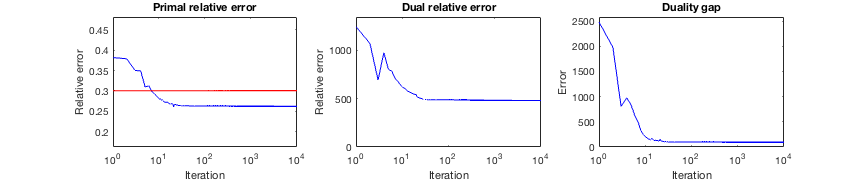
\includegraphics[scale=0.6]{noisy_random_signal_relative_errors_stagnate}
\caption{Primal relative error (\ref{Eqn:term_crit-candidate_residuals}d), dual relative error (\ref{Eqn:term_crit-candidate_residuals}b), and duality gap (\ref{Eqn:term_crit-candidate_residuals}f) for 10,000 iterates of Algorithm \ref{Alg:PGD} applied to a natural noise model with $n=16$, $L=6$ observations, and noise ratio $0.30$.  The horizontal axis is log-plotted to highlight early progress along with later stagnation.  The pair $(X_\star, y_\star)$ are computed with \texttt{SDPT3}.}
\label{Fig:noisy_random_relative_errors_stagnate}
\end{figure}
% experiments.figure.noisyrandom_relative_errors_stagnate


Figure \ref{Fig:noisy_random_relative_errors_stagnate} demonstrates that Algorithm \ref{Alg:PGD} stagnates when attempting to solve a PLGD model with Gaussian noise (\ref{Eqn:PhaseLift-GD_Gaussian_noise}).  In this problem, primal feasibility (\ref{Eqn:saga_conv_crit_primal}) is acheived at iterate 6, and further progress is made over the following early iterations, as indicated by the primal relative error (\ref{Eqn:term_crit-candidate_residuals}d) plot.  However, the strong duality condition (\ref{Eqn:saga_conv_crit_gap}) is never satisfied, and the final duality gap at iterate 10,000 is 97.63.  Likewise, the dual variable $y_k$ does not approach the optimal dual variable $y_\star$, as indicated by the dual relative error (\ref{Eqn:term_crit-candidate_residuals}b) plot.  In this particular PLGD model, $X_\star$ is rank three, causing the dual objective $\lambda_1(\caA^*y)$ to be nondifferentiable near $y_\star$ per Corollary \ref{Cor:PLGD-optimality} (e).  Thus Algorithm \ref{Alg:PGD} identifies the dual objective $\lambda_1(\caA^*y)$ as nondifferentiable at iterate 84 reverts to the monotone stepsize sequence (\ref{Eqn:GD-steplength}).  


The next experiment establishes that PLGD models with Gaussian noise (\ref{Eqn:PhaseLift-GD_Gaussian_noise}) almost always have an optimal matrix $X_\star$ with rank greater than one, and this rank problem causes the stagnation of Algorithm \ref{Alg:PGD}.  Table \ref{Tab:average_rank_soln_matrix_with_gaussian_dual_variable} compares PLGD models with synthetic (\ref{Eqn:PhaseLift-GD_synthetic_noise}) and Gaussian noise (\ref{Eqn:PhaseLift-GD_Gaussian_noise}), depicting the rank of the optimal matrix $X_\star$ and the behavior of Algorithm \ref{Alg:PGD}.

\begin{table}[H]
\centering 
\begin{tabular}{ |cc|c|c|c|c|c|c| }
\hline
	\multicolumn{2}{|c|}{} &	\multicolumn{3}{c|}{Synthetic noise} 	&	\multicolumn{3}{c|}{Gaussian noise}  \\
\multicolumn{2}{|c|}{}  	&	\multicolumn{1}{c}{$L = 4$}	&	\multicolumn{1}{c}{$L = 6$}	&	\multicolumn{1}{c|}{$L = 8$} &	\multicolumn{1}{c}{$L = 4$}	&	\multicolumn{1}{c}{$L = 6$}	&	\multicolumn{1}{c|}{$L = 8$}		\\
\hline
& $\textnormal{rank}(X_\star)$
	&	1	&	1	&	1	&	3.41 	&	3.28 	&	3.27 \\
$\epsilon_\rel = 0.05$ &	 Algo. \ref{Alg:PGD} itns.
	&	125.09	&	144.20 & 182.26	&	1,000	&	1,000	&	1,000\\
& 	duGap
	&	$1.17_{-4}$  &  $1.18_{-4}$ &  $1.18_{-4}$ 	&	9.60   & 3.88   & 3.86\\
\hline
& $\textnormal{rank}(X_\star)$
	&	1	&	1	&	1	&	2.99 	&	3.00 &	3.04 \\
$\epsilon_\rel = 0.15$ &	 Algo. \ref{Alg:PGD} itns.
	&	62.48  & 85.32 &  95.58	&	1,000	&	1,000	&	1,000\\
& 	duGap
	&	$1.20_{-4}$ &  $1.35_{-4}$ &  $1.33_{-4}$ &	15.9 &  14.0 &  15.8 \\
\hline
& $\textnormal{rank}(X_\star)$
	&	1	&	1	&	1	&	2.64  	&	2.70  &	2.89\\
$\epsilon_\rel = 0.30$ &	 Algo. \ref{Alg:PGD} itns.
	&	40.34  & 50.88  & 64.28	&	1,000	&	1,000	&	1,000\\
& 	duGap
	&	$1.17_{-4}$ &  $1.23_{-4}$ &  $1.27_{-4}$		&	   21.2 &  26.7  & 31.5\\
 \hline
\end{tabular}

\caption{Algorithm \ref{Alg:PGD} results and optimal matrix rank for PLGD models with synthetic (\ref{Eqn:PhaseLift-GD_synthetic_noise}) and Gaussian noise (\ref{Eqn:PhaseLift-GD_Gaussian_noise}).  This table depicts the mean rank of $X_\star$, number of Algorithm \ref{Alg:PGD} iterations, and final duality gap (\ref{Eqn:term_crit-candidate_residuals}f) (duGap) for 100 random phase retrieval models with signal size $n=16$, noise ratio $\epsilon_\rel$, and oversampling $L$.  In all synthetic noise models (\ref{Eqn:PhaseLift-GD_synthetic_noise}), the solution $X_\star$ was rank-one and Algorithm \ref{Alg:PGD} converged.  In all Gaussian noise models (\ref{Eqn:PhaseLift-GD_Gaussian_noise}), the algorithm reached the maximum of 1,000 iterations without attaining the termination condition (\ref{Eqn:saga_conv_crit_gap}).  Note that pairs $(X_\star, y_\star)$ are computed with \texttt{SDPT3} and numbers $n_{-k}$ are shorthand for $n \times 10^{-k}$.} \label{Tab:average_rank_soln_matrix_with_gaussian_dual_variable}
\end{table}
% experiments.table.noisyrandom_mean_rank_lifted_signal_exact_solution


Table \ref{Tab:average_rank_soln_matrix_with_gaussian_dual_variable} demonstrates that PLGD models with Gaussian noise (\ref{Eqn:PhaseLift-GD_Gaussian_noise}) typically have optimal matrices with rank greater than one, causing Algorithm \ref{Alg:PGD} to stagnate.  
Algorithm \ref{Alg:PGD} cannot attain an optimal primal matrix $X_\star$ with rank greater than one because the primal recovery (\ref{Eqn:GD-primal_rec2}) and refinement (\ref{Eqn:GD-PFD}) steps used in this algorithm only return a rank-one matrix $X = xx^*$.  
Additionally, Corollary \ref{Cor:PLGD-optimality}, (e) indicates that $\text{rank}(X_\star)$ is a lower bound on the multiplicity of the algebraically largest eigenvalue of $\caA^*y_\star$.  
Thus the objective function $\lambda_1(\caA^*y)$ will be nondifferentiable in some neighborhood around $y_\star$ and Algorithm \ref{Alg:PGD} will stagnate prior to approaching $y_\star$.  
As a result, Algorithm \ref{Alg:PGD} cannot attain a pair $(X,y)$ that are sufficiently close to the optimal pair $(X_\star, y_\star)$ and fails to satisfy the duality gap condition (\ref{Eqn:saga_conv_crit_gap}).


In contrast to the Gaussian models (\ref{Eqn:PhaseLift-GD_Gaussian_noise}), we see that PLGD models with synthetic noise (\ref{Eqn:PhaseLift-GD_synthetic_noise}) consistenly have rank-one optimal matrices $X_\star$, allowing Algorithm \ref{Alg:PGD} to converge.  
Each synthetic noise model (\ref{Eqn:PhaseLift-GD_synthetic_noise}) in Table \ref{Tab:average_rank_soln_matrix_with_gaussian_dual_variable} had an optimal dual matrix $\caA^*y_\star$ with a unique algebraically largest eigenvalue, making the dual objective function $\lambda_1(\caA^*y)$ differentiable at $y_\star$ and allowing Algorithm \ref{Alg:PGD} to approach the optimal dual variable $y_\star$.  
Once the pair $(X,y)$ are sufficiently close to the optimal pair, the duality gap condition (\ref{Eqn:saga_conv_crit_gap}) is met and convergence is declared.
At this point, the primal recovery equation (\ref{Eqn:PLGD-noise_is_dual_variable}) successfully denoises the noisy observation $b = \mathbf{b} + \epsilon y_\star / ||y_\star||_2$ because the synthetic noise steps (\ref{Def:synthetic_noise}) guarantee an exact relation $\eta = \epsilon y_\star / ||y_\star||_2$ between the noise term $\eta$ and optimal dual variable $y_\star$.
Thus Algorithm \ref{Alg:PGD} is able to return a matrix $X$ which accurately approximates the optimal matrix $X_\star = \mathbf{x}\mathbf{x}^*$.  










Table \ref{Tab:average_rank_soln_matrix_with_gaussian_dual_variable} also helps to explain why dual refinement (Algorithm \ref{Alg:PGD}, step 13) is not beneficial for PLGD models with Gaussian noise (\ref{Eqn:PhaseLift-GD_Gaussian_noise}).  As we saw in Table \ref{Tab:noiseless_runtimes}, an inaccurate signal $x$ can cause the dual refinement problem (\ref{Eqn:GD-DFP}) to return an unreliable update $\hat{y}$.  Figure \ref{Fig:noisy_random_DFP_vs_no_DFP} depicts the progress made by Algorithm \ref{Alg:PGD} with and without dual refinement for three PLGD models with Gaussian noise (\ref{Eqn:PhaseLift-GD_Gaussian_noise}).

\begin{figure}[H]
\hbox{\hspace{-1.0cm}  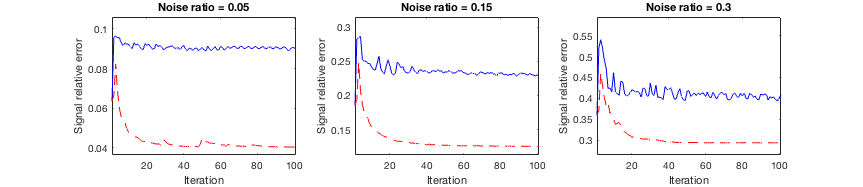
\includegraphics[scale=0.6]{noisy_random_signal_DFP_vs_no_DFP}}
\caption{A comparison of Algorithm \ref{Alg:PGD} with and without dual refinement (\ref{Eqn:GD-DFP}) for PLGD models with Gaussian noise (\ref{Eqn:PhaseLift-GD_Gaussian_noise}) with various noise levels, with random Gaussian signal of size $n = 128$ and $L = 10$ observations.  The solid blue line indicates dual refinement, and the dashed red line indicates no dual refinement.}
\label{Fig:noisy_random_DFP_vs_no_DFP}
\end{figure}
% experiments.figure.noisyrandom_dual_refinement_fails



Figure \ref{Fig:noisy_random_DFP_vs_no_DFP} demonstrates that the dual refinement step (\ref{Eqn:GD-DFP})  inhibits the progress otherwise made by Algorithm \ref{Alg:PGD}.  This step is initialized with a signal $x$ which corresponds to the rank-one matrix iterate $X = xx^*$.  Since the optimal matrix $X_\star$ tends to have rank greater than one, the dual refinement problem (\ref{Eqn:GD-DFP}) will not be properly initialized and may return a poor update $\hat{y}$.  Thus the dual refinement step in Algorithm \ref{Alg:PGD} is not beneficial for signal recovery in phase retrieval problems with Gaussian noise (\ref{Eqn:phase_retrieval_Gaussian_noise}).





\section{New Termination Conditions}  	\label{Subsec:PLGD_term_crit-new_term_crit}


In Section \ref{Subsec:PLGD_term_crit-stagnation}, we saw that Algorithm \ref{Alg:PGD} tends to stagnate when solving phase retrieval problems with Gaussian noise (\ref{Eqn:phase_retrieval_Gaussian_noise}), failing to satisfy the duality gap termination condition (\ref{Eqn:saga_conv_crit_gap}) original established in \cite{DBLP:journals/siamsc/FriedlanderM16}.  
This section establishes new termination conditions for Algorithm \ref{Alg:PGD} for PLGD models with Gaussian noise (\ref{Eqn:PhaseLift-GD_Gaussian_noise}) and demonstrates the effectiveness of these conditions for identifying stagnation of Algorithm \ref{Alg:PGD}.  
(For a comparison of the unused residuals from (\ref{Eqn:term_crit-candidate_residuals}), see Appendix \ref{Sec:Appx-further_reasons_for_new_term_crit}.)







We begin by presenting the new termination conditions for Algorithm \ref{Alg:PGD} for PLGD models with Gaussian noise (\ref{Eqn:PhaseLift-GD_Gaussian_noise}).  To identify stagnation of Algorithm \ref{Alg:PGD} and declare termination, the primal difference (\ref{Eqn:term_crit-candidate_residuals}e) is set to 
\begin{equation}
	\label{Eqn:term_crit_new-primal_difference}
\frac{| \rho - \hat{\rho} |}{\rho} \leq  \textnormal{tol}_\textnormal{primal} = 10^{-5}, \ \ \rho = ||\caA(xx^*) - b||_2
\end{equation}
and the dual variable difference (\ref{Eqn:term_crit-candidate_residuals}i) is set to
\begin{equation}
	\label{Eqn:term_crit_new-dual_difference}
\frac{||y- \hat{y}||_2}{||y||_2} \leq \textnormal{tol}_\textnormal{dual}= 10^{-4},
\end{equation}
where a hat indicates the previous iterate (e.g., $\hat{y} = y_{k-1}$).  Termination is declared when (\ref{Eqn:term_crit_new-primal_difference}) and (\ref{Eqn:term_crit_new-dual_difference}) are satisfied or after a maximum of 300 iterations are performed.  After termination, the signal returned corresponds to the signal among the previous 20 with the smallest duality gap (\ref{Eqn:term_crit-candidate_residuals}f) value.  










To demonstrate the effectiveness of these termination conditions, we consider a set of six PLGD models with Gaussian noise (\ref{Eqn:PhaseLift-GD_Gaussian_noise}) solved with Algorithm \ref{Alg:PGD}.   The signal relative error (\ref{Eqn:term_crit-candidate_residuals}a) serves as a control measurement to identify when Algorithm \ref{Alg:PGD} has stagnated and should terminate.  Figure \ref{Fig:term_crit-signal_err} depicts the signal relative error (\ref{Eqn:term_crit-candidate_residuals}a) for each of these models.


\newpage

\begin{figure}[H]
\centering
\hbox{\hspace{-1.2cm} 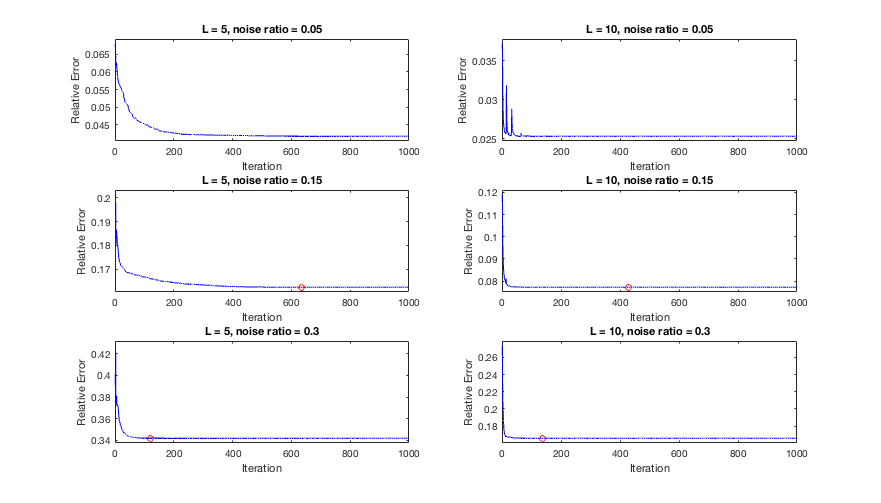
\includegraphics[scale=0.6]{term_crit-signal_err} }\vspace{-0.4cm}
\caption{Signal relative errors (\ref{Eqn:term_crit-candidate_residuals}a) for six PLGD models with Gaussian noise (\ref{Eqn:PhaseLift-GD_Gaussian_noise})  solved with Algorithm \ref{Alg:PGD}. The image in Figure \ref{Fig:parrot_signal_iterates} was resized to $64 \times 64$ pixels, made grayscale, and six models were generated with oversampling rates of $L = 5, 10$ and noise ratios $\epsilon_\rel = 0.05, 0.15, 0.30$.  These models were then solved using Algorithm \ref{Alg:PGD} set to terminate after 1,000 iterations.  The red circle (where present) indicates when the dual objective was determined nondifferentiable.}
\label{Fig:term_crit-signal_err}
\end{figure}
% experiments.figure.noisyimage_new_termination_criteria

Figure \ref{Fig:term_crit-signal_err} depicts the early progress and quick stagnation of Algorithm \ref{Alg:PGD} for these PLGD models with Gaussian noise (\ref{Eqn:PhaseLift-GD_Gaussian_noise}).  For each model, virtually no measurable progress was made after iteration 500.  Yet the point at which each model stagnates appears to differ, and in one case ($L = 10$ and $\epsilon_\rel = 0.05$) the signal quality appears to vary greatly for neighboring iterates.  Thus we examine the behavior in Figure \ref{Fig:term_crit-signal_err} to identify the desired interval of iterates in which Algorithm \ref{Alg:PGD} should terminate for each model.




The results in Figure \ref{Fig:term_crit-signal_err} suggest that models with a larger oversampling rate and those with a larger noise ratio make progress faster and stagnate earlier.  One indicator that the point of stagnation differs for these models is the point at which Algorithm \ref{Alg:PGD} identifies the objective function $\lambda_1(\caA^*y)$ as nondifferentiable (i.e., the condition (\ref{Eqn:GD-diff_tol}) fails).  The models in Figure \ref{Fig:term_crit-signal_err} with the least noise never identified a nondifferentiable objective, whereas the noisiest models identified nondifferentiable objectives very early (at iterate 122 for $L=5$ and 137 for $L=10$).  Another indicator that the models of Figure \ref{Alg:PGD} stagnate at different rates is the point at which the primal objective is found to be feasible, as described in Table \ref{Tab:term_crit-pr_feas_faster_for_big_L_noise}.

\begin{table}[H]
\centering
\begin{tabular}{ |c|c|c| }
\hline
&	$L = 5$
	&	$L = 10$	\\
 \hline
$\epsilon_\rel = 0.05$
&     33 &   3 		\\
 \hline
$\epsilon_\rel = 0.15$
&  N/A &  3 	\\
 \hline
$\epsilon_\rel = 0.30$
&  22 &  3	\\
 \hline
\end{tabular}
	\caption{Iterate at which Algorithm \ref{Alg:PGD} became primal feasible for models from Figure \ref{Fig:term_crit-signal_err}.}
	\label{Tab:term_crit-pr_feas_faster_for_big_L_noise}
\end{table}
% experiments.figure.noisyimage_new_termination_criteria

Table \ref{Tab:term_crit-pr_feas_faster_for_big_L_noise} shows that all three models with oversampling $L = 10$ found feasible signals after just 3 iterations, yet the models with $L = 5$ were a bit slower, and in particular the model with $L = 5$ and $\epsilon_\rel = 0.15$ never identified a feasible signal.


Based on these observations, Table \ref{Tab:term_crit-desired_termination_windows} proposes iterate intervals in which Algorithm \ref{Alg:PGD} appears to have stagnated for each model in Figure \ref{Fig:term_crit-signal_err}, providing a guideline for assessing the new termination conditions (\ref{Eqn:term_crit_new-primal_difference}) and (\ref{Eqn:term_crit_new-dual_difference}).
\begin{table}[H]
\centering
\begin{tabular}{ |c|c|c| }
\hline
&	$L = 5$
	&	$L = 10$	\\
 \hline
$\epsilon_\rel = 0.05$
&     200-400 &   50-200 		\\
 \hline
$\epsilon_\rel = 0.15$
&  200-400 &  50-100 	\\
 \hline
$\epsilon_\rel = 0.30$
&  100-200 &  50-100	\\
 \hline
\end{tabular}
	\caption{Intervals of iterates at which Algorithm \ref{Alg:PGD} appears to stagnate for models from Figure \ref{Fig:term_crit-signal_err}.}
	\label{Tab:term_crit-desired_termination_windows}
\end{table}







In order to demonstrate that the primal difference (\ref{Eqn:term_crit-candidate_residuals}e) and dual variable difference (\ref{Eqn:term_crit-candidate_residuals}i) are accurate indicators of the stagnation of Algorithm \ref{Alg:PGD}, Figure \ref{Fig:term_crit-pr_and_dual} depicts the behavior of these residuals for the models in Figure \ref{Fig:term_crit-signal_err}.  
Note that the vertical axis indicates specific tolerances and the horizontal axis indicates the first iterate at which Algorithm \ref{Alg:PGD} would satisfy this tolerance.


\begin{figure}[H]
\centering
\hbox{\hspace{-1.4cm} 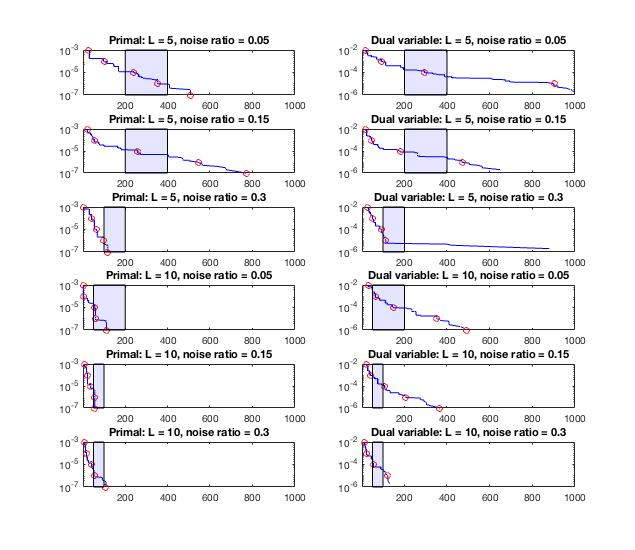
\includegraphics[scale=0.6]{term_crit-pr_and_dual} }\vspace{-1.3cm}
\caption{Plots of tolerance values against the iterate at which Algorithm \ref{Alg:PGD} first satisfies this tolerance for the models discussed in Figure \ref{Fig:term_crit-signal_err}.  Tolerances depicted are difference values for the primal objective (\ref{Eqn:term_crit-candidate_residuals}e) and dual variable (\ref{Eqn:term_crit-candidate_residuals}i).  Red circles are placed at tolerances $10^{-n}$.  The blue rectangles indicate the proposed intervals of termination from Table \ref{Tab:term_crit-desired_termination_windows}.}
\label{Fig:term_crit-pr_and_dual}
\end{figure}
% experiments.figure.noisyimage_new_termination_criteria



For each of the models in Figure \ref{Fig:term_crit-pr_and_dual}, the termination conditions (\ref{Eqn:term_crit_new-primal_difference}) and (\ref{Eqn:term_crit_new-dual_difference}) are satisfied within or close to each respective interval of stagnation from Table \ref{Tab:term_crit-desired_termination_windows}.  For the models with oversampling $L = 5$, Algorithm \ref{Alg:PGD} satisfies the tolerances $\tol_\textnormal{primal} = 10^{-5}$ from (\ref{Eqn:term_crit_new-primal_difference}) and $\tol_\textnormal{dual} = 10^{-4}$ from (\ref{Eqn:term_crit_new-dual_difference}) within or slightly prior to each respective desired interval.  Likewise, Algorithm \ref{Alg:PGD} achieve these desired tolerances for the models with $L =10$ within or slightly after each desired interval.  As an additional precaution, the maximum iteration count of 300 iterates will prevent running Algorithm \ref{Alg:PGD} after it has stagnated.

Note that there is also theoretical justification for selecting the dual variable difference (\ref{Eqn:term_crit-candidate_residuals}i) as a termination condition.  Proposition \ref{Prop:PLGD-opt_unconstrained} showed that the variable $y$ is optimal for the PLGD model (\ref{Eqn:PhaseLift-P-GD}) if $y = \Pi_\caC(y - \alpha g)$ for some $g \in \partial f(y)$ and all $\alpha > 0$.  This property corresponds to the termination condition 
\begin{equation*}
|| \Pi_\caC(y - \alpha g) - y ||_2 \leq \text{tol}.
\end{equation*}
If we make this condition relative by setting $\text{tol} = 10^{-4}||\Pi_\caC(y - \alpha g)||_2$, then we recover the new dual variable difference condition (\ref{Eqn:term_crit_new-dual_difference}).






One additional concern for termination conditions is the nonmonotonic nature of Algorithm \ref{Alg:PGD}.  In Figure \ref{Fig:term_crit-signal_err}, the model with $L = 10$ and $\epsilon_\rel = 0.05$ demonstrates that Algorithm \ref{Alg:PGD} may produce neighboring signal iterates with varying accuracy.  Since this algorithm is nonmonotonic and relies on a subroutine to recover the current approximate signal, the accuracy of the sequence of recovered signals can vary dramatically.  Thus we need a reliable indicator to select a sufficiently accurate signal among the previous iterates.  Figure \ref{Fig:term_crit-duality_gap} depicts the signal relative error (\ref{Eqn:term_crit-candidate_residuals}a) and duality gap (\ref{Eqn:term_crit-candidate_residuals}f) for the $L = 10$, $\epsilon_\rel = 0.05$ model.  Note that the new termination conditions $\tol_\text{primal} = 10^{-5}$ and $\tol_\text{dual} = 10^{-4}$ would select the 148th iterate as the candidate solution.  



\begin{figure}[H]
\centering
\hbox{\hspace{-1.7cm} 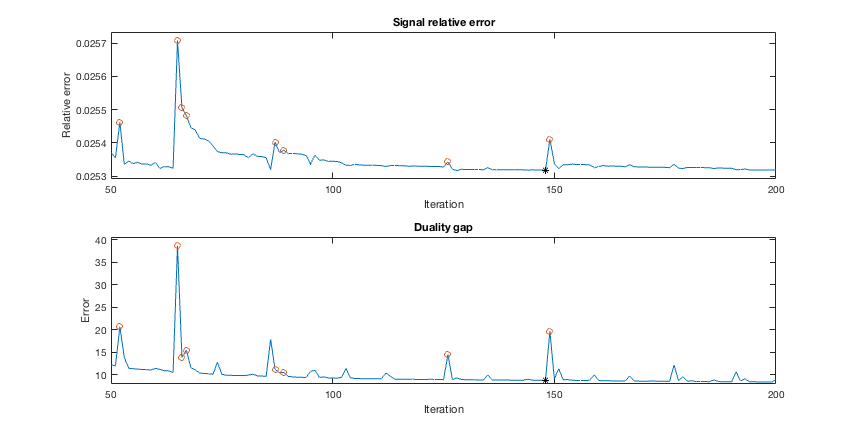
\includegraphics[scale=0.6]{term_crit-duality_gap} }
\caption{Signal relative error (\ref{Eqn:term_crit-candidate_residuals}a) and duality gap (\ref{Eqn:term_crit-candidate_residuals}f) for the model from Figure \ref{Fig:term_crit-signal_err} with oversampling $L = 10$ and noise ratio $\epsilon_\rel = 0.05$. Red circles indicate signals with relative error at least $0.05\%$ above the mean of their ten neighbors, and the black asterisk indicates both the final iterate based on new termination conditions and the optimal iterate based on minimum duality gap.}
\label{Fig:term_crit-duality_gap}
\end{figure}

% experiments.figure.noisyimage_new_termination_criteria



Figure \ref{Fig:term_crit-duality_gap} demonstrates that the duality gap (\ref{Eqn:term_crit-candidate_residuals}f) violation closely matches the signal relative error (\ref{Eqn:term_crit-candidate_residuals}a).  Among the previous iterates, those with the least accurate signal (indicated by the red circle) are accurately identified as having a duality gap value greater than the minimum (black asterisk).  Thus once Algorithm \ref{Alg:PGD} terminates, we select the signal among the last 20 with the lowest duality gap value.








Given the new termination conditions (\ref{Eqn:term_crit_new-primal_difference}), (\ref{Eqn:term_crit_new-dual_difference}), the maximum iteration count of 300, and the signal selection method discussed above, the Figure \ref{Fig:term_crit-model_term_for_tols} depicts the iterate at which Algorithm \ref{Alg:PGD} would terminate for each PLGD model with Gaussian noise from Figure \ref{Fig:term_crit-signal_err}.

\begin{figure}[H]
\centering
\hbox{\hspace{-1.9cm} 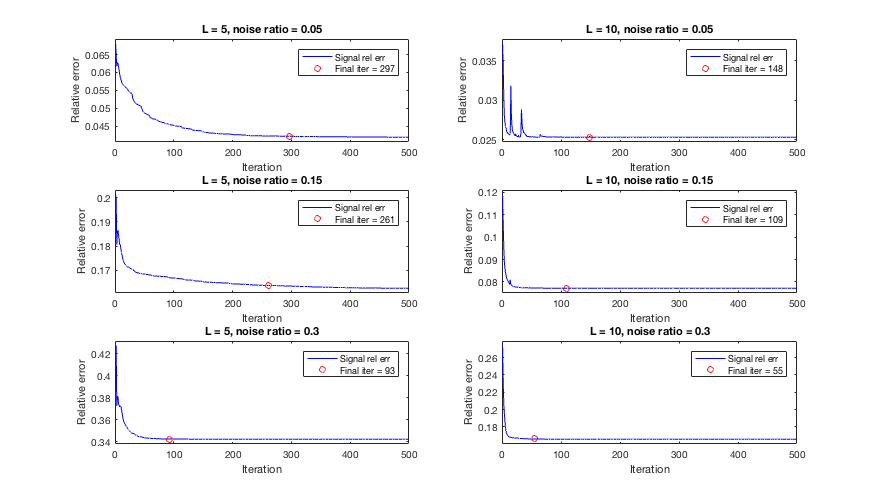
\includegraphics[scale=0.6]{term_crit-model_term_for_tols} }\vspace{-0.4cm}
	\caption{Iterate at which Algorithm \ref{Alg:PGD} terminates for the models from Figure \ref{Fig:term_crit-signal_err} based on new termination conditions.}
\label{Fig:term_crit-model_term_for_tols}
\end{figure}
% experiments.figure.noisyimage_new_termination_criteria

For each model in Figure \ref{Fig:term_crit-model_term_for_tols}, Algorithm \ref{Alg:PGD} successfully terminates within or nearby the interval of stagnation established in Table \ref{Tab:term_crit-desired_termination_windows}.
Given the new termination conditions (\ref{Eqn:term_crit_new-primal_difference}) and (\ref{Eqn:term_crit_new-dual_difference}), we may now treat Algorithm \ref{Alg:PGD} as a black-box method for noisy phase retrieval and examine the sequence of eigenvalue problems generated by Algorithm \ref{Alg:PGD}.




